\documentclass[8pt,a5paper]{extarticle}
%\documentclass[9pt,a5paper]{extarticle}
%\usepackage[margin=.75in]{geometry}
\usepackage[margin=.8cm]{geometry}
%\usepackage[margin=1in]{geometry}
\usepackage[utf8]{inputenc}
\usepackage[IL2]{fontenc}
\usepackage[czech]{babel}
\usepackage{microtype}
\usepackage{amssymb}
\usepackage{amsthm}
\usepackage{amsmath}
\usepackage{xcolor}
\usepackage{graphicx}
\usepackage{wasysym}
\usepackage{multicol}

\usepackage[inline]{enumitem}

\newcommand{\R}{\mathbb{R}}

\newcommand{\hint}[1]{{\color{gray}\footnotesize\noindent(Nápověda: #1)}}

\setlist[enumerate]{label={(\alph*)},topsep=\smallskipamount,itemsep=\smallskipamount,parsep=0pt,itemjoin={\quad}}
\setlist[itemize]{topsep=\smallskipamount,noitemsep}

\def\tisk{%
\newbox\shipouthackbox
\pdfpagewidth=2\pdfpagewidth
\let\oldshipout=\shipout
\def\shipout{\afterassignment\zdvojtmp \setbox\shipouthackbox=}%
\def\zdvojtmp{\aftergroup\zdvoj}%
\def\zdvoj{%
    \oldshipout\vbox{\hbox{%
        \copy\shipouthackbox
        \hskip\dimexpr .5\pdfpagewidth-\wd\shipouthackbox\relax
        \box\shipouthackbox
    }}%
}}%

\let\results\newpage
\let\endresults\relax

\def\resultssame{%
    \long\def\results##1\endresults{%
        %\vfill
        \noindent\rotatebox{180}{\vbox{##1}}%
    }%
}


\newtheorem*{poz}{Pozorování}

\theoremstyle{definition}
\newtheorem{uloha}{\atr Úloha}
\newtheorem{suloha}[uloha]{\llap{$\star$ }Úloha}
\newtheorem*{bonus}{Bonus}
\newtheorem*{defn}{Definice}

\pagestyle{empty}

\let\ee\expandafter

\def\vysld{}
\let\printvysl\relax

\makeatletter
\long\def\vyslplain#1{\ee\ee\ee\gdef\ee\ee\ee\vysld\ee\ee\ee{\ee\vysld\ee\printvysl\ee{\the\c@uloha}{#1}}}
\let\vysl\vyslplain

\def\locvysl#1{\ee\gdef\ee\locvysld\ee{\locvysld\item #1}}
\let\lv\locvysl

\newenvironment{ulohav}[1][]{\begin{uloha}[#1]\gdef\locvysld{\begin{enumerate*}}}{\ee\vyslplain\ee{\locvysld\end{enumerate*}}\end{uloha}}
\def\stitem{\@noitemargtrue\@item[$\star$ \@itemlabel]}

\makeatother

\def\atr{}
\def\basic{\def\atr{\llap{\mdseries$\sun$ }\gdef\atr{}}}
\def\interest{\def\atr{\llap{$\star$ }\gdef\atr{}}}
\def\iinterest{\def\atr{\llap{$\star\star$ }\gdef\atr{}}}


\begin{document}


\section*{29. Opáčko před čtvrtletkou}


\begin{uloha} % státní maturita
\[ 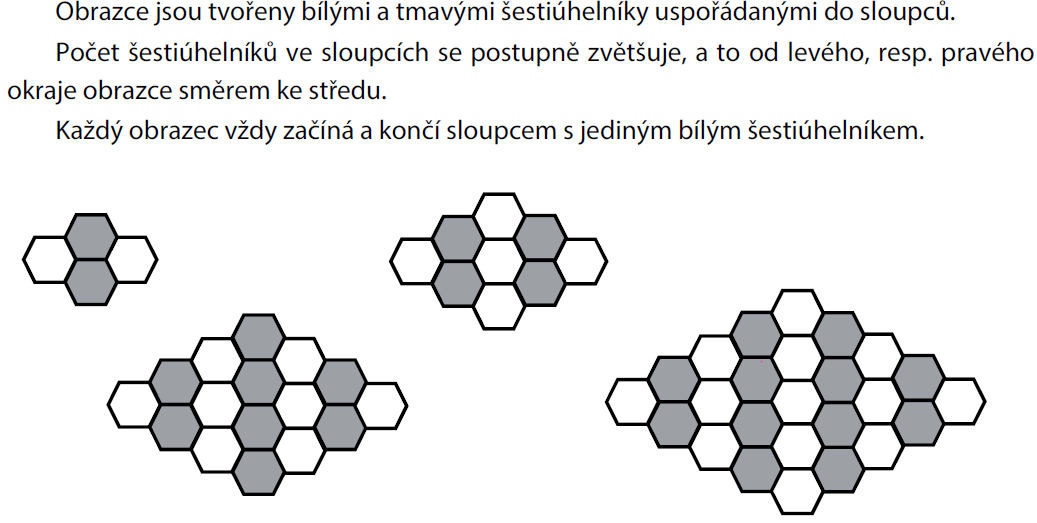
\includegraphics[width=.6\hsize]{uly.png} \]
V jednom z dalších obrazců je v \textbf{nejdelším} sloupci 59 šestiúhelníků nad sebou. Určete, kolik je v onom obrazci \textbf{bílých} šestiúhelníků.\vysl{1741}
\end{uloha}

\begin{ulohav}
Megasněhulák se skládá z $n$ sněhových koulí, přičemž poloměr každé koule je vždy $\frac34$ poloměru koule pod ní. \textbf{Druhá} koule odspodu má poloměr 1\,m. Určete \textbf{objem} celého sněhuláka, pokud se skládá z \begin{enumerate}\item $n=20$ koulí,\lv{$(\frac43)^4 \pi \frac{(\frac34)^{60}-1}{(\frac34)^{3}-1}$} \item $n=\infty$ koulí.\lv{$(\frac43)^4 \pi \frac{1}{1-(\frac34)^{3}}$}\end{enumerate} (Připomenutí: objem koule o poloměru $r$ je $V = \frac43 \pi r^3$. Napovím, že objemy koulí tvoří geom. posloupnost.)
\end{ulohav}

\begin{uloha} % státní maturita
\[ 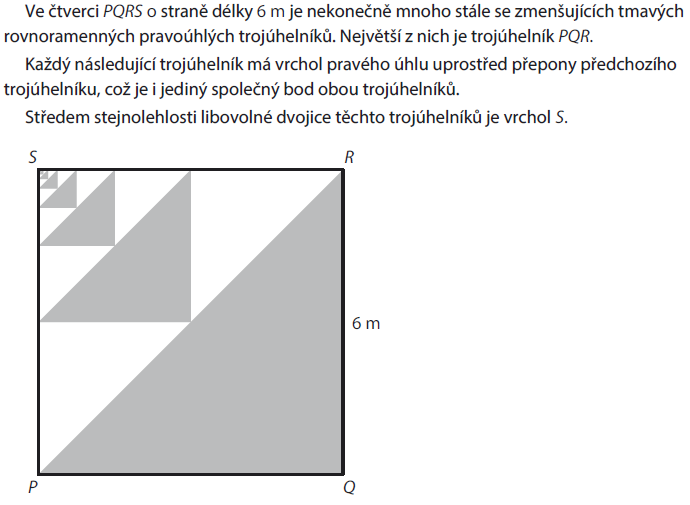
\includegraphics[width=.65\hsize]{trojuh.png} \]
Určete celkový obsah šedé oblasti. \vysl{24}
\end{uloha}

\begin{ulohav}
U následujících řad určete, pro která $x \in \R$ konvergují, a potom jejich součet (který zjednodušte):
\begin{enumerate*}
\everymath{\displaystyle}
\item $\sum_{k=1}^\infty (x^2-2)^k$\lv{$x \in (-\sqrt3;-1)\cup (1;\sqrt3)$, $\frac{2-x^2}{x^2-3}$}
\item $\sum_{k=1}^\infty \left(\frac{x+1}x\right)^k$\lv{$x \in (-\infty;-\frac12)$, $-1-x$}
\item $\sum_{k=1}^\infty x^{3k}$\lv{$x \in (-1;1)$, $\frac{x^3}{1-x^3}$}
\end{enumerate*}
\end{ulohav}

\interest
\begin{ulohav}
Určete součet následujících řad (které \textbf{nejsou geometrické}):
\begin{enumerate}
\everymath{\displaystyle}
\item $\sum_{n=0}^\infty \frac{n}{2^n}$\lv{2} \hint{např. $\frac{3}{2^3} = \frac1{2^3}+\frac1{2^3}+\frac1{2^3}$}
\item $\sum_{n=1}^\infty \frac{1}{n(n+1)}$\lv{1} \hint{přepište sčítaný zlomek na rozdíl dvou zlomků}
\end{enumerate}
\end{ulohav}


\baselineskip=1.25\baselineskip
\setlist[enumerate]{label=\textbf{(\alph*)},itemjoin={\quad}}

\results
\parindent=0pt
\parskip=\smallskipamount
\rightskip=0pt plus1fil\relax
\def\printvysl#1#2{\textbf{#1.} #2\par}
\vysld
\endresults


\end{document}